%
% File acl2016.tex
%
%% Based on the style files for ACL-2015, with some improvements
%%  taken from the NAACL-2016 style
%% Based on the style files for ACL-2014, which were, in turn,
%% Based on the style files for ACL-2013, which were, in turn,
%% Based on the style files for ACL-2012, which were, in turn,
%% based on the style files for ACL-2011, which were, in turn, 
%% based on the style files for ACL-2010, which were, in turn, 
%% based on the style files for ACL-IJCNLP-2009, which were, in turn,
%% based on the style files for EACL-2009 and IJCNLP-2008...

%% Based on the style files for EACL 2006 by 
%%e.agirre@ehu.es or Sergi.Balari@uab.es
%% and that of ACL 08 by Joakim Nivre and Noah Smith

\documentclass[11pt]{article}
\usepackage{acl2016}
\usepackage{times}
\usepackage{url}
\usepackage{latexsym}
\usepackage[hidelinks]{hyperref}
\usepackage{graphicx}
\usepackage{float}

%\aclfinalcopy % Uncomment this line for the final submission
%\def\aclpaperid{***} %  Enter the acl Paper ID here

%\setlength\titlebox{5cm}
% You can expand the titlebox if you need extra space
% to show all the authors. Please do not make the titlebox
% smaller than 5cm (the original size); we will check this
% in the camera-ready version and ask you to change it back.

\newcommand\BibTeX{B{\sc ib}\TeX}

\title{Building predictors for the game mia}
%nur sichtbar in finaler submission.
\author{First Author \\
  Affiliation / Address line 1 \\
  Affiliation / Address line 2 \\
  Affiliation / Address line 3 \\
  {\tt email@domain} \\\And
  Alexander Diegel \\
  Affiliation / Address line 1 \\
  Affiliation / Address line 2 \\
  Affiliation / Address line 3 \\
  {\tt email@domain} \\}

\date{}

\begin{document}
\maketitle
\begin{abstract}
  This term paper deals with the topic of predicting different artificial intelligence approaches based on the game mia. It starts with an short introduction to artificial intelligence. Then, the description of the game mia on which the project is based on. Afterwards, the strategies of the different implemented artificial intelligences (AI) are explained. It follows an explanation of our approach predicting the behavior of the different AIs. Finally, the results of the experiments are discussed.
  %TODO weiteres?
\end{abstract}


\section{Introduction}
Artificial intelligence has become an increasingly important field in computer science and other areas such as automotive (self-driving cars) or security (face-detection).
In computer games artificial intelligence reaches new stages of success (Google bot AlphaGo for the game go). In this term paper we now want to answer the question if it is possible to predict different artificial intelligence approaches based on the game mia. The main achievement would be the accuracy of correct predictions if a player (AI) will to lie or tells the correct value. If the actual value is lesser or greater seems not as important as prediction liars properly. 
%TODO noch mehr?



\section{The Game}
Mia is a simple dice game that is played with two dices and a flat bottomed container (or a dice cup). At the beginning each player has a certain amount of lives (e.g. five).
The first player rolls the dices but keeps their values hidden from the other players. He then can decide if he wants to tell the truth to the next player and announce a value that was was actually rolled. Alternatively he can lie and announce a greater or lesser value than the rolled one.
But each player has to announce a greater value than the previous player.

The next player (who still has not seen the actual values) can now believe the passer, call the passer a liar and look on the dice or pass the dice to the next player (still without looking) announcing a higher value. 

A player looses a life if he called the previous one a liar and looked on the values to find out that they are what the previous player has announced or even higher. Otherwise the previous player looses a life. 

The higher value of the roll is multiplied by then and then added to the other die (a 4 and a 2 is 42). 
The \textbf{scoring} is from highest to lowest:  21 (Mia), 11, 22, 33, 44, 55, 66, 65, 64, 63, 62, 61, 54, 53, 52, 51, 43, 42, 41, 32, 31.

If a player announces mia the next player either believes him, give up (without looking at the dices) and looses one life. Or he may look at the dice. If it was actually mia then he looses two lifes if it was not, the previous player looses a life. (For further information see \cite{mia:2016}.)

\section{The Strategies}

\subsection{Statistic Approach}
\subsection{Approach with certain degree of randomness}
\subsection{A SVM learning approach}

\section{The predictor}
To predict the different strategical approaches we used a support vector machine (SVM) predictor with radial basis functions. A linear predictor would not have been sufficient due to the complexity of data, but with the SVM-predictor adequate results could be expected.
By using SVM we are interested in separating two (or more) classes by a separating hyperplane with maximal margin. The margin is defined with respect to the training points as the minimal distance between the hyperplane and a training point.(See \cite{luxburg:2016} and \cite[187--227]{Schoellkopf:02}.)

\section{Discussion of results}

\begin{figure}[H]
	\centering
	
\includegraphics[width=.45\textwidth]{../testdata/svm1.png}
	\caption{caption svm1}
	\label{svm1}
\end{figure}
\begin{figure}[H]
	\centering
	
\includegraphics[width=.45\textwidth]{../testdata/svm2.png}
	\caption{caption svm2}
	\label{svm2}
\end{figure}
\begin{figure}[H]
	\centering
	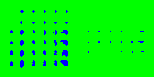
\includegraphics[width=.45\textwidth]{../testdata/svm3.png}
	\caption{caption svm3}
	\label{svm3}
\end{figure}
\begin{figure}[H]
	\centering
	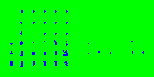
\includegraphics[width=.45\textwidth]{../testdata/svm4.png}
	\caption{caption svm4}
	\label{svm4}
\end{figure}
\begin{figure}[H]
	\centering
	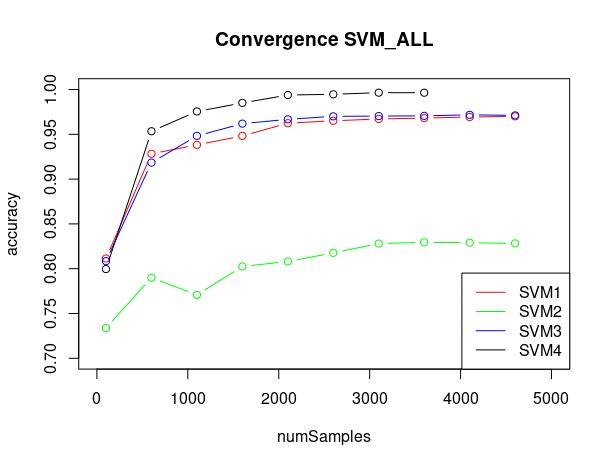
\includegraphics[width=.45\textwidth]{../testdata/convergence_all.png}
	\caption{caption convergence all}
	\label{convergence all svms}
\end{figure}
\begin{figure}[H]
	\centering
	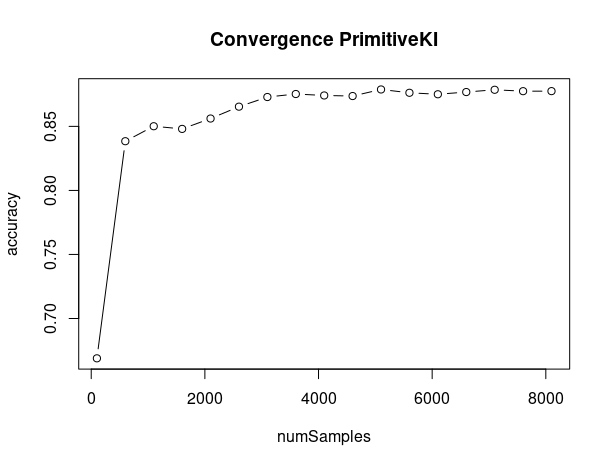
\includegraphics[width=.45\textwidth]{../testdata/conv_prim.png}
	\caption{caption convergence all}
	\label{convergence primitive}
\end{figure}
\begin{figure}[H]
	\centering
	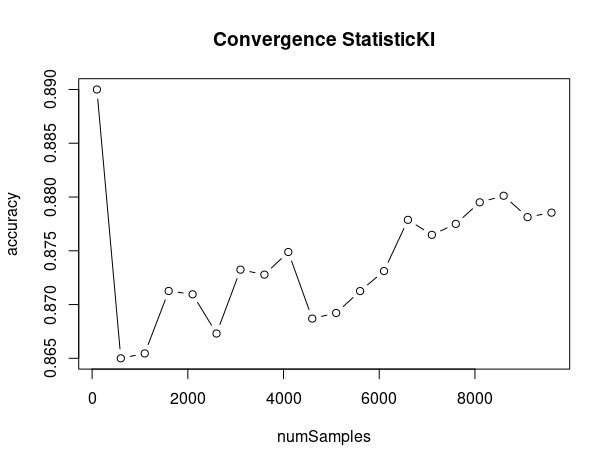
\includegraphics[width=.45\textwidth]{../testdata/conv_stat.png}
	\caption{caption convergence all}
	\label{convergence statistic}
\end{figure}

%10000 for stat und prim
%5000 for svms

%\begin{table}
%\centering
%\small
%\begin{tabular}{cc}
%\begin{tabular}{|l|l|}
%\hline
%{\bf Command} & {\bf Output}\\\hline
%\verb|{\"a}| & {\"a} \\
%\verb|{\^e}| & {\^e} \\
%\verb|{\`i}| & {\`i} \\ 
%\verb|{\.I}| & {\.I} \\ 
%\verb|{\o}| & {\o} \\
%\verb|{\'u}| & {\'u}  \\ 
%\verb|{\aa}| & {\aa}  \\\hline
%\end{tabular} & 
%\begin{tabular}{|l|l|}
%\hline
%{\bf Command} & {\bf  Output}\\\hline
%\verb|{\c c}| & {\c c} \\ 
%\verb|{\u g}| & {\u g} \\ 
%\verb|{\l}| & {\l} \\ 
%\verb|{\~n}| & {\~n} \\ 
%\verb|{\H o}| & {\H o} \\ 
%\verb|{\v r}| & {\v r} \\ 
%\verb|{\ss}| & {\ss} \\\hline
%\end{tabular}
%\end{tabular}
%\caption{Example commands for accented characters, to be used in, e.g., \BibTeX\ names.}\label{tab:accents}
%\end{table}



%\penalty -5000

%We suggest that instead of
%\begin{quote}
%  ``\cite{Gusfield:97} showed that ...''
%\end{quote}
%you use
%\begin{quote}
%``Gusfield \shortcite{Gusfield:97}   showed that ...''
%\end{quote}




\section*{Acknowledgments}

The acknowledgments should go immediately before the references.  Do
not number the acknowledgments section. Do not include this section
when submitting your paper for review.

% include your own bib file like this:
%\bibliographystyle{acl}
%\bibliography{acl2016}
\bibliography{acl2016}
\bibliographystyle{acl2016}
\appendix

\section{Supplemental Material}
\label{sec:supplemental}
%ACL 2016 also encourages the submission of supplementary material
%to report preprocessing decisions, model parameters, and other details
%necessary for the replication of the experiments reported in the 
%paper. Seemingly small preprocessing decisions can sometimes make
%a large difference in performance, so it is crucial to record such
%decisions to precisely characterize state-of-the-art methods.
%
%Nonetheless, supplementary material should be supplementary (rather
%than central) to the paper. It may include explanations or details
%of proofs or deriations that do not fit into the paper, lists of
%features or feature tempates, sample inputs and outputs for a system,
%pseudo-code or source code, and data. (Source code and data should
%be separate uploads, rather than part of the paper).
%
%The paper should not rely on the supplementary material: while the paper
%may refer to and cite the supplementary material will be available to the
%reviewers, they will not be asked to review the
%supplementary material.
%
%Appendices (i.e. supplementary material in the form of proofs, tables,
%or pseudo-code) should come after the references, as shown here. Use
%\verb|\appendix| before any appendix section to switch the section
%numbering over to letters.


\end{document}
